\subsection{Comparison of Entropy, Snooze and DVMS}
\label{subsec:first-usecase}

\MS{From Euro-Par: to be extended and rewritten}

%\AL{Il faudra parler du nombre de migrations qui est egalement une
%  métrique pertinente. Plusieurs algorithms tentent de reduire cette
%  metrique }
%\AL[AL]{Il faudra mettre des snapshots de PajeNG}
% Evaluation of VMPlaceS on Grid'5000: simulations were running on one server.
As a validation of our approach (and a contribution by itself), we now
provide simulation results comparing the Entropy, Snooze and DVMS
strategies.
% Due to space limitations we present a generaly study
% analyzing the violation times as well as the
% duration of the computation and reconfiguration phases. However, we
% highlight that such a study enables us to investigate some variant and possible
% improvements of Snooze and DVMS that made possible to easily study  thanks to
% \vmps.

\subsubsection{Experimental Conditions.}

%\emph{Experimental conditions. ~}
% All simulations have been performed on the Lyons-based clusters of the
% Grid'5000 testbed.
Each simulation has been executed on a dedicated server, thus
avoiding interferences between simulations and ensuring
reproducibility between the different invocations.
% Scripts: automation of the deployment, running of simulations and the collect
% of results.
% It enables us to run a large number of simulations, with several variants
% of the scheduling algorithm.
%
\vmps has been configured to simulate a homogeneous infrastructure of
PMs composed of 8 cores, 32~GB of RAM and 1~Gpbs Ethernet NIC. To
enable a fair comparison between the three strategies, the scheduling
resolver only considered 7 cores, \ie one was devoted to run the
Snooze LC or the DVMS admin processes (a common experimental setup).
% Dedicating one core for the host OS and other administrative processes
% is something which is rather usual and thus we believe acceptable in
% our experimental methodology.
Ten VMs have been initially launched on each simulated PM. Each VM
relied on one of the VM classes described in the accuracy experiment
and one set of load-change parameters has been used: $\lambda$ =
\#VMs/300, $\mu = 60$ and $\sigma = 20$. The stationary state was
reached after 20 min of the simulated time with a global cluster load
of 85\%.
%as depicted in Fig. \ref{fig:load_figure}.
% To accelerate the simulations, we have chosen to limit the
We have performed simulations over a period of 1800 seconds. The
consolidation ratio, \ie the number of VMs per node, has been defined
such that a sufficient number of violations is generated. We have
discovered that below a global load of 75\%, few VM violations occurred
under the selected Gaussian distribution we have chosen. This result
is rather satisfactory as it can explained why most production DCs
target a comparable load
level.\footnote{\url{http://www.cloudscaling.com/blog/cloud-computing/amazons-ec2-generating-220m-annually/}}
Finally, infrastructures composed of 128, 256, 512 and 1024 PMs,
hosting respectively 1280, 2560, 5120 and 10240 VMs have been
investigated. For Entropy and Snooze that rely on service nodes,
additional simulated PMs have been provided. For Snooze, one GM has
been created per 32 LCs (\ie PMs). The solver has been invoked
every 30s for Entropy and Snooze.
% We remind that no service node had to be provisioned for DVMS as a
% DVMS process has been executed directly on top of each hosting node.
%
% In order to cope with real DC conditions, we defined the parameters
% for node crashes to simulate a fault on average every 6 months for a
% duration of 300 seconds. These values correspond to the Mean Time To
% Failure (MTTF) and the Mean Time To Repair (MTTR) of a Google DC
% server~\cite[pp. 107-108]{datacenterAsComputer}. We underline that at
% the scale we performed our simulations such a crash ratio was not
% sufficient to impact the behavior of the scheduling policies.
% Dedicated simulations were mandatory to study the influence of node
% crashes. However, due to the space limitations, we do not present them
% in the article and only gives major trends. Regarding Entropy,
% although the lost of the service node can be critic, the failure
% probability is so small that the single point of failure issue can be
% easily solved by a fail-over approach. Regarding Snooze, the heartbeat
% strategy enables the reconstruction of the hierarchy in a relative
% short time and thus crashes on service nodes do not significantly
% impact the resolution of violations (in our case less than 10 seconds
% is mandatory to reorganize the Snooze topology with a 6 seconds
% heartbeat mechanism). Finally regarding DVMS, the crash of one node
% does not have any impact of the resolution has the composition of the
% microcosm is reevaluated immediately.
%%
%Finally, we highlight that all configuration files used to perform the discussed simulations can
%be downloaded from the \vmps repository.

\subsubsection{General  Analysis.}
\label{subsec:general-comparison}

% \begin{figure}
% \subcapcentertrue
% \subfigure[Infrastructure load]{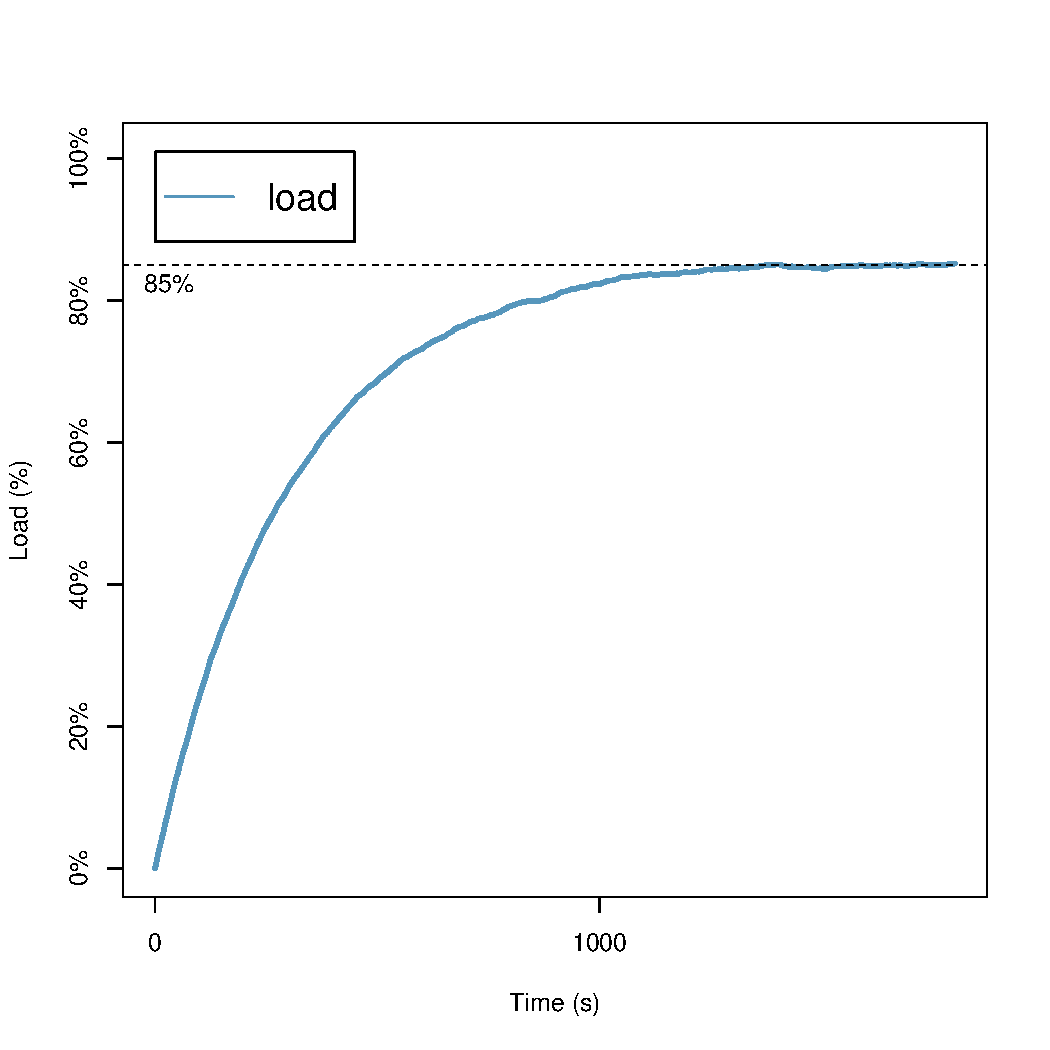
\includegraphics[width=4cm]{./figures/experiments/1024-hierarchical.pdf}\label{fig:load_figure}}
% \subfigure[Cumulated Violation Time]{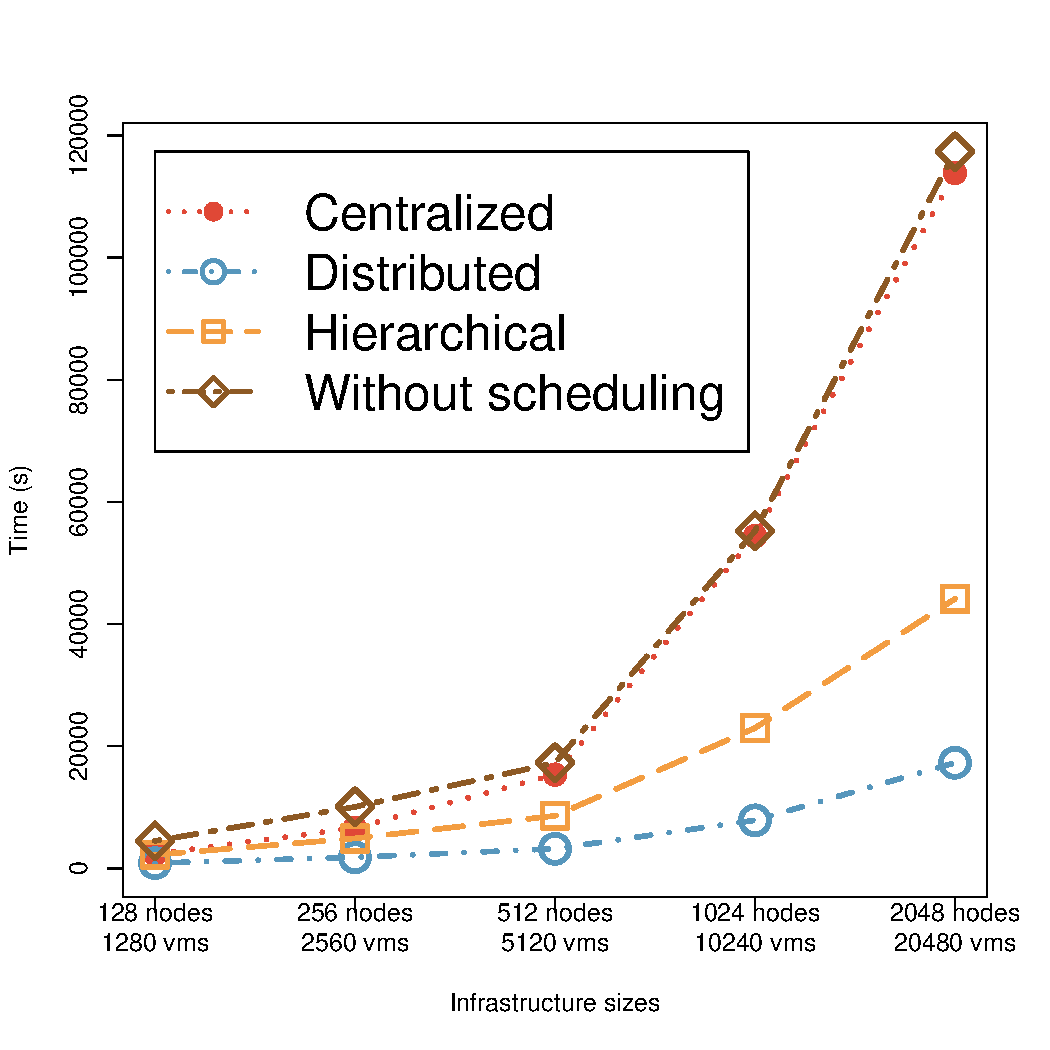
\includegraphics[width=4cm]{./figures/experiments/violation_time.pdf}\label{fig:cumulated_violation}}
% \caption{Simulation Results - 10 VMs per node (VM load: $\mu=60$ and $\sigma=20$)}
% \label{fig:simulation-overview}
% \end{figure}

\begin{figure*}[t]
\subcapcentertrue
\subfigure{
  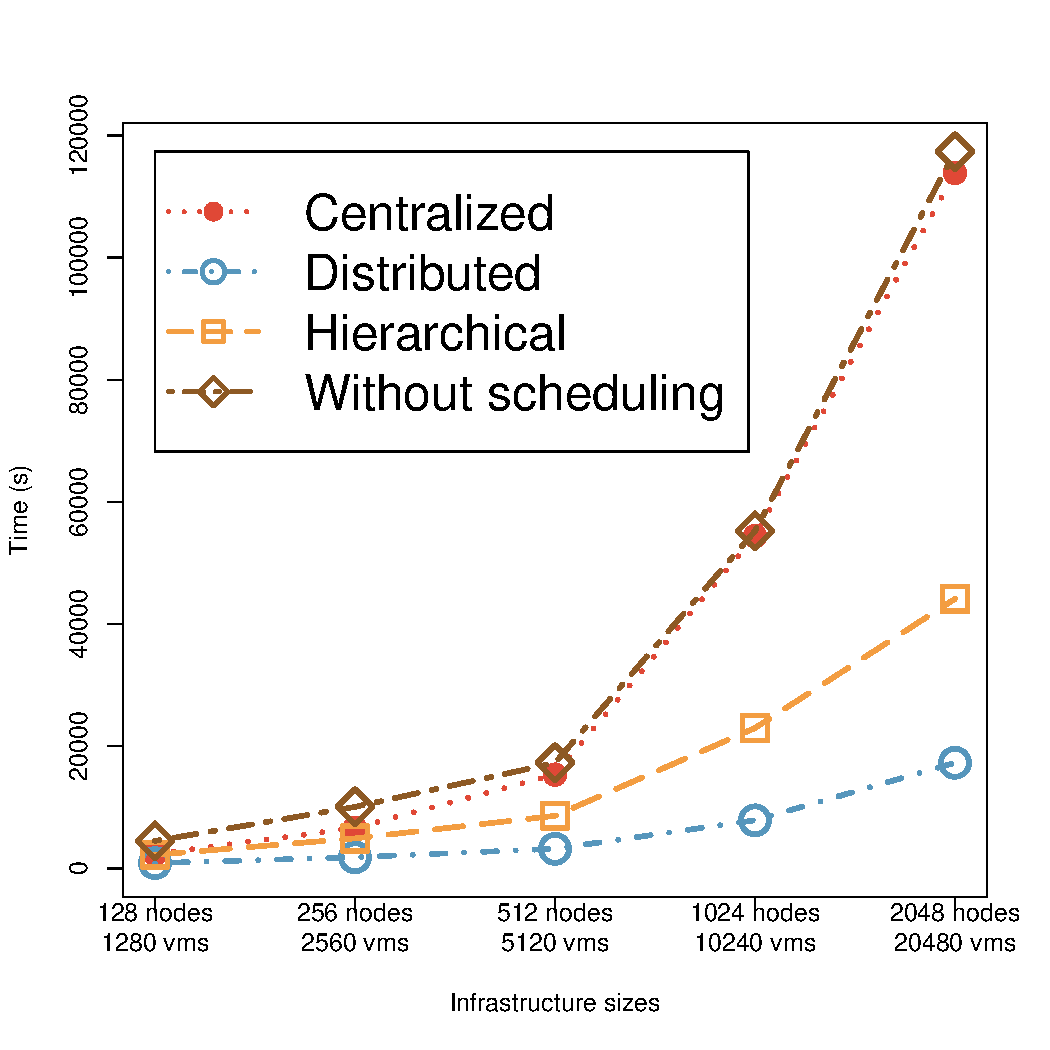
\includegraphics[width=.46\textwidth]{figures/experiments/violation_time.pdf}
  \label{fig:violation_time}}
\begin{minipage}{.5\textwidth}
\centering

%\subfigure[Duration of violation ($med \pm \sigma$)]{
\subfigure{
    {\tiny \begin{tabular}{|P{17mm}@{\:}||@{\:}c@{\:}|@{\:}c@{\:}|@{\:}c@{\:}|}
      \thickhline
      \textbf{Infrastructure size}
        & \multicolumn{3}{c@{\:}|}{Duration of \textbf{violations}
          ($\mu \pm \sigma$)}
          \Tstrut \\
         \hfill  & ~Centralized~ & ~Hierarchical~ & Distributed \Bstrut \\
      \thickhline
        128 nodes   & 21.26 $\pm$ 13.55 & 21.07 $\pm$ 12.32 &   9.55 $\pm$ 2.57 \\
        256 nodes   & 40.09 $\pm$ 24.15 & 21.45 $\pm$ 12.10 &   9.58 $\pm$ 2.51 \\
        512 nodes   & 55.63 $\pm$ 42.26 & 24.54 $\pm$ 16.95 &   9.57 $\pm$ 2.67 \\
        1024 nodes  & 81.57 $\pm$ 86.59 & 29.01 $\pm$ 38.14 & \:9.61 $\pm$ 2.54
      \Rstrut  \\ \hline
      \thickhline
  \end{tabular} }
%\label{table:detailed_violation_time}
}

%\subfigure[Duration of computations ($\mu \pm \sigma$)]{
\subfigure{
    {\tiny \begin{tabular}{|P{17mm}@{\:}||@{\:}c@{\:}|@{\:}c@{\:}|@{\:}c@{\:}|}
      \thickhline
      \textbf{Infrastructure size}
        & \multicolumn{3}{c@{\:}|}{Duration of \textbf{computations}
          ($\mu \pm \sigma$)}
          \Tstrut \\
         \hfill  & ~Centralized~ & ~Hierarchical~ & Distributed \Bstrut \\
      \thickhline
        128 nodes   &  3.76 $\pm$  7.43 &  2.52 $\pm$  4.63 &   0.29 $\pm$ 0.03 \\
        256 nodes   &  7.97 $\pm$ 15.03 &  2.65 $\pm$  4.69 &   0.25 $\pm$ 0.02 \\
        512 nodes   & 15.71 $\pm$ 29.14 &  2.83 $\pm$  4.98 &   0.21 $\pm$ 0.01 \\
        1024 nodes  & 26.41 $\pm$ 50.35 &  2.69 $\pm$  4.92 & \:0.14 $\pm$ 0.01
      \Rstrut  \\ \hline
      \thickhline
  \end{tabular} }
%\label{table:detailed_computation_time}
}

%\subfigure[Duration of reconfigurations ($\mu \pm \sigma$)]{
\subfigure{
    {\tiny \begin{tabular}{|P{17mm}@{\:}||@{\:}c@{\:}|@{\:}c@{\:}|@{\:}c@{\:}|}
      \thickhline
      \textbf{Infrastructure size}
        & \multicolumn{3}{c@{\:}|}{Duration of \textbf{reconfigurations}
          ($\mu \pm \sigma$)}
          \Tstrut \\
         \hfill  & ~Centralized~ & ~Hierarchical~ & Distributed \Bstrut \\
      \thickhline
        128 nodes   & 10.34 $\pm$  1.70 &  10.02 $\pm$  0.14 &   10.01 $\pm$ 0.11 \\
        256 nodes   & 10.26 $\pm$  1.45 &  10.11 $\pm$  0.83 &   10.01 $\pm$ 0.08 \\
        512 nodes   & 11.11 $\pm$  3.23 &  10.28 $\pm$  1.50 &   10.08 $\pm$ 0.82 \\
        1024 nodes  & 18.90 $\pm$  7.57 &  10.30 $\pm$  1.60 & \:10.04 $\pm$ 0.63
      \Rstrut  \\ \hline
      \thickhline
  \end{tabular} }
%\label{tab:detailed_reconf_time}
}
\end{minipage}
\caption{Scalability/Reactivity analysis of Entropy, Snooze and DVMS}
\label{fig:general-comparison}
\end{figure*}

%\emph{Simulation results and analysis. ~}
Figure~\ref{fig:general-comparison} presents on the left the cumulated
violation time for each placement policy and on the right several
tables that give more details by presenting the mean and the standard
deviations of the duration of, respectively, the violations and the
computation/reconfiguration phases. As anticipated, the centralized
approach did not scale and even incurs an overhead in the largest
scenario compared to a system that did not perform any dynamic
scheduling. The more nodes Entropy has to monitor, the less efficient
it is during both the computation and reconfiguration phases.
% Regarding the computation, the VMPP is a NP-Hard problem and thus it
% is not surprising that it takes more time to resolve larger
% problems.
This is to be expected for the computation phase (which tries to
tackle an NP-complete problem).  As to reconfiguration,
% as Entropy has to solve much more violations simultaneously,
the reconfiguration plan becomes more complex for large scenarios,
including several migrations coming from and going to the same
nodes. Such plans are not optimal as they increase the bottleneck
effects at the network level of each involved PM. Such a simulated
result is valuable as it confirms that reconfiguration plans should
avoid such manipulations as much as possible.
%
The results of the hierarchical approach are clearly better than the
Entropy-based ones but worse than those using DVMS-based
placement. However, diving into the details, we can see that both the
time needed for the computation and reconfiguration are almost
independent from the cluster size (around~3s and~10s) and not much
worse than those of DVMS, especially for the reconfiguration phase,
which is predominant. These results can be easily explained: the
centralized policy addresses the VMPP by considering all nodes at each
invocation, while the hierarchical and the distributed algorithms
divide the VMPP into sub problems, considering smaller numbers of
nodes (32~PMs in Snooze and, on average, 4 in the case of DVMS). To
clarify the influence of the group size on the performance of Snooze,
\ie the ratio of LCs attached to one GM, we have performed additional
simulations for varying group sizes.  \vmps has significantly
facilitated this study as the corresponding simulations differ just by
configuration parameters and do not require modifications to the code
base.

